\documentclass[12pt, twosides]{report}

\usepackage{graphicx}
\graphicspath{ {figures/} }
\usepackage[left=2.5cm,right=2cm,top=2.5cm]{geometry}


\usepackage[utf8]{inputenc}
\usepackage{t1enc}
\usepackage[magyar]{babel}
\linespread{1.5}

\usepackage{footnote}
\usepackage{subfigure}
\usepackage{float}
\usepackage[]{algorithm2e}
\usepackage{amsmath}
\usepackage{mathptmx}
\usepackage{pdfpages}

\usepackage{xcolor}
\usepackage{hyperref}
\hypersetup{
    colorlinks,
    linkcolor=black,
    citecolor=black,
	urlcolor={blue!80!black},
	unicode=true
}
% 
\urlstyle{same}

\usepackage{listings}
\definecolor{dkgreen}{rgb}{0,0.6,0}
\definecolor{gray}{rgb}{0.5,0.5,0.5}
\definecolor{mauve}{rgb}{0.58,0,0.82}
\definecolor{light-gray}{gray}{0.25}

\lstdefinestyle{yaml}{	
	backgroundcolor=\color{white}, % choose the background color;
	basicstyle=\fontsize{8}{8}\ttfamily,% the size of the fonts that are used for the code
	breakatwhitespace=false, % sets if automatic breaks should only happen at whitespace
	breaklines=true, % sets automatic line breaking
	commentstyle=\color{dkgreen},  % comment style
	deletekeywords={...},  % if you want to delete keywords from the given language
	escapeinside={\%}{)},  % if you want to add LaTeX within your code
	extendedchars=true,  % lets you use non-ASCII characters; for 8-bits encodings only, does not work with UTF-8
	frame=none,	 	 % adds a frame around the code
	keepspaces=true, % keeps spaces in text, useful for keeping indentation of code (possibly needs columns=flexible)
	keywordstyle=\color{blue}\bfseries, % keyword style
	otherkeywords={*,...}, % if you want to add more keywords to the set
	numbers=none,  % where to put the line-numbers; possible values are (none, left, right)
	numbersep=5pt, % how far the line-numbers are from the code
	numberstyle=\tiny\color{gray}, % the style that is used for the line-numbers
	rulecolor=\color{black}, % if not set, the frame-color may be changed on line-breaks within not-black text (e.g. comments (green here))
	showspaces=false,% show spaces everywhere adding particular underscores; it overrides 'showstringspaces'
	showstringspaces=false,  % underline spaces within strings only
	showtabs=false,  % show tabs within strings adding particular underscores
	%stepnumber=1,  % the step between two line-numbers. If it's 1, each line will be numbered
	stringstyle=\color{mauve}, % string literal style
	tabsize=2,
	columns=fullflexible  % Using fixed column width (for e.g. nice alignment)
	sensitive = true,
	morekeywords={name, runs-on, on, jobs, build, run, steps, uses}
}
\lstset{style=yaml}

\title{
	{Bőrdaganatok felismerése}\\
	{\large Sapientia\\
	Erdélyi Magyar Tudományegyetem, Marosvásárhely}
}
\author{
	Fábián, Ervin\\
	\texttt{fabian.ervin@student.ms.sapientia.ro}
	\and
	Iclănzan, David Andrei\\
	\texttt{iclanzan@ms.sapientia.ro}	
}
\date{2025}

%%%%%%%%%%%%%%%%%%%%%%%%%%%%%%%%%%%%%%%%%%%%%%%%%%%%%%%%%%%%%%%%%%%%%%%%%
\begin{document}

%
\includepdf[pages={1,2,3}]{pdfs/allamvizsga_borito.pdf}

%\section*{Extras}
%Extract

\textbf{Cuvinte cheie}: 

%\pagebreak

%
\includepdf[pages={6}]{pdfs/allamvizsga_borito.pdf}

%\section*{Kivonat}
%Kivonat

\textbf{Kulcsszavak}: 
%\pagebreak

%\section*{Abstract}
%Abstract

\textbf{Keywords}: 
%\pagebreak

\pagenumbering{gobble}

\tableofcontents

\listoffigures

\chapter{Bevezető}
\pagenumbering{arabic}
\section{Bevezető}
A bőr felületén lévő elváltozások igen változatosak. Diagnosztikailag az egyik
legfontosabb megkülönböztetési szempont az elváltozás daganatos jellege vagy 
annak hiánya.
Mesterséges intelligencia általi osztályozása bőrelváltozásoknak igéretes eredményeket 
ért el, de a szelekciós torzitás (a klinikailag malignusnak ítélt elváltozásoknak 
dokumentálása jellemző), a magas színtű szakmai ismeret szűkségessége és a csak nagy
részletességű dermaszkópiai felvételek használatával voltak lehetséges.
Ezek behatárolták ezen osztályozási kisérletek hatékonyságát.

Éppen ezért célunk egy olyan weboldal létrehozása amely okostelefonok elváltozásokról
készített képei alapján is, valamilyen valószínűséggel meg tudja határozni, hogy egy
bizonyos elváltozást érdemes szakemberrel kivizsgáltatni.

 A \ref{fig:child_dragged} ábrán látható ahogy egy robotraj együttesen elmozdít egy kislányt.

\begin{figure}[h]
    \centering
    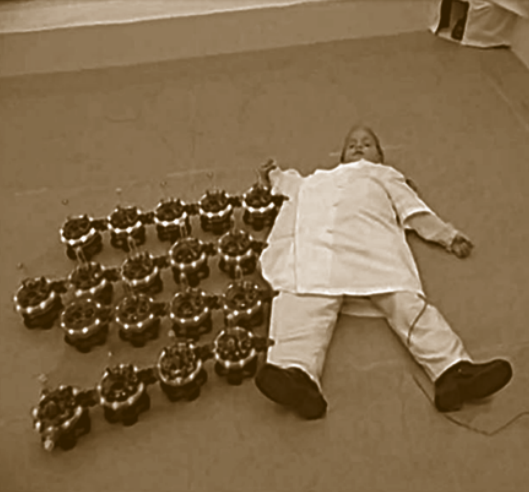
\includegraphics[scale=0.6]{figures/images/literature/child_dragged_robots.png}
    \caption{Rövid szöveg a képről, hivatkozás \cite{parker2016multiple}}
    \label{fig:child_dragged}
\end{figure}

\section{Cím 2}

Két ábra egymás mellett (lásd \ref{fig:insbots} ábra).

\begin{figure}[h]
    \centering
    \hfill
    \subfigure[Insbot \cite{colot2004insbot}]{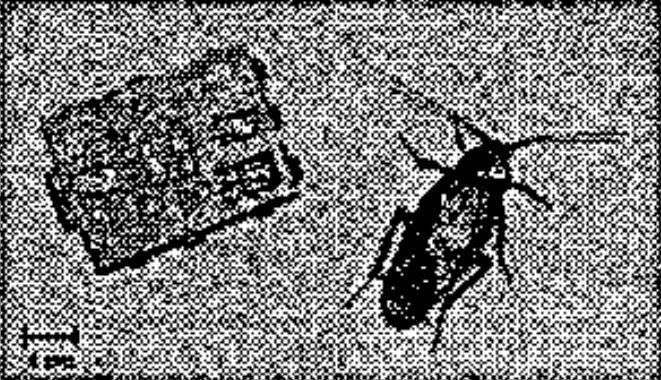
\includegraphics[scale=0.3]{figures/images/literature/insbot.png}}
    \hfill
    \subfigure[Insbot és csótányok interakciója \cite{garnier2011ants}.]{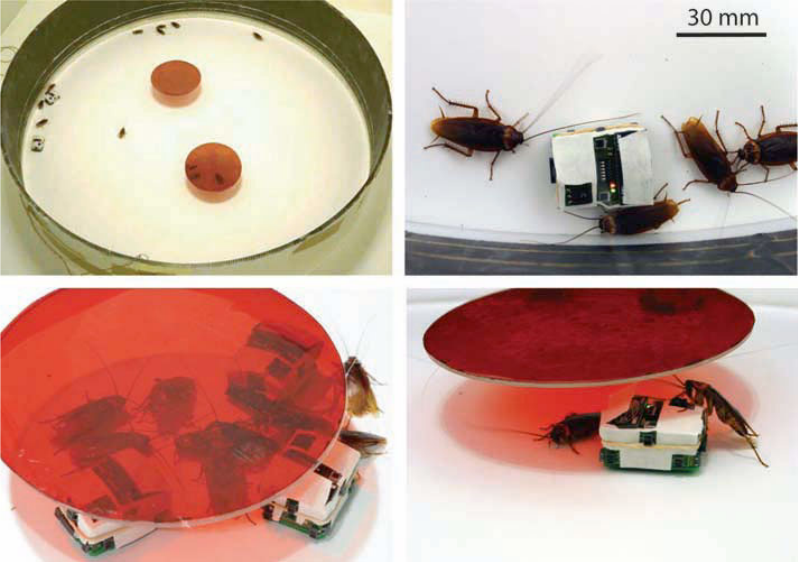
\includegraphics[scale=0.25]{figures/images/literature/insbot_cockroach.png}}
    
    \caption{Insbot és csótányok interakciója. Az insbot-ok képesek a csótányokat csalogatni.}
    \label{fig:insbots}
\end{figure}

\chapter{Szakirodalom áttekintése}
\section{Cím 1}

\subsection{Alcím 1}

Táblázat: 

\begin{figure}[h]
    \begin{table}[H]
    \begin{footnotesize}
        \begin{center}
            \begin{tabular}{p{2.5cm}|p{3.5cm}|p{4cm}|p{4cm}}
            \textbf{Kritériumok}                    & V\-rep                              & ARGoS  & Gazebo \\
            \hline         
            Ingyenes                            & Igen, van fizetős verzió is         & Igen             & Igen \\
            \hline         
            Absztrakciós szint                  & Valósághű         & Emelkedett absztrakciós szintet ajánl             & Valósághű  \\
            \hline         
            Robotrajokra optimalizált           & Nem optimalizált         & Teljesen optimalizált           & Képes, nagyobb erőforrásigény, mint az ARGOS-nak  \\
            \hline         
            Nyílt forráskódú                    & Igen         & Igen            & Igen  \\
            \hline         
            Támogatott programozási nyelvek     & C/C++, Python, Java, Lua, Matlab, Octave          & C/C++ és Lua             & C/C++  \\
            \hline         
            Valós robotok modelljei             & Igen          & Igen             & Igen  \\
            \end{tabular}
        \end{center}
    \end{footnotesize}
    \end{table}
    \label{table:simulators}
    \caption{V-REP, ARGoS, Gazebo összehasonlítása}
\end{figure}

Hivatkozás a táblázatra: \ref{table:simulators}

\chapter{Elméleti áttekintés}
\section{Elméleti áttekintés}

Pszeudokód: 

\begin{algorithm}[h]
    \begin{small}
    \KwData{Tanulási tényező ($\alpha \in (0, 1])$), $\epsilon > 0$}
    Véletlenszerű érték minden $Q_{1}(s,a)$ és $Q_{2}(s,a)$-nek, kivéve $Q($terminális$, \cdot ) = 0$, $s \in S$, $a \in A$ \;
    \For{minden epizód}{
        S inicalizálása\;
        \Repeat{S terminális állapot}{
        $A \leftarrow$ cselekvés, $S$ állapotban $\epsilon$-greedy szerint $Q_{1}+Q_{2}$ \;
        $A$ cselekedet végrehajtása, R és S' megfigyelése\;
        \eIf{ $50\%$ eséllyel}
            {$Q_{1}(S, A) \leftarrow Q_{1}(S, A) + \alpha [R + \gamma Q_{2}(S', arg\max_{a}Q_{1}(S', a)) - Q_{1}(S, A)]$}
            {$Q_{2}(S, A) \leftarrow Q_{2}(S, A) + \alpha [R + \gamma Q_{1}(S', arg\max_{a}Q_{2}(S', a)) - Q_{2}(S, A)]$}
        $S \leftarrow S'$\;
        }
    }
    \end{small}
    \caption{Dupla Q-tanulás \cite{sutton2018reinforcement}.}        
    \label{algo:double_q}
\end{algorithm}


Hivatkozás pszeudokódra: \ref{algo:double_q}.

\chapter{Rendszer specifikációi}
\section{Cím 1}

%Terv
\chapter{Gyakorlati megvalósítás} \label{chpt:implementation}
\section{Ágensek vezérlése}

\textbf{Hivatkozásra példa}

Az ágensek vezérléséhez a potenciálmező navigációs módszer volt felhasználva. Ez egy bevált módszer a robotrajok vezérléséhez \cite{szanto2015investigation}. Az alapötlete, hogy az akadályok taszító erővel hatnak az ágensre és a cél vonzó erővel. Ennek a két erőnek az eredője határozza meg az irányt amerre érdemes haladni.

\subsection{Potenciálmező navigáció}

\textbf{Egyenletekre példa}

A potenciálmező navigációs módszernél az erők nagysága az \eqref{eq:poti} egyenlet szerint van kiszámolva.

\begin{equation}
    \left\{
    \begin{array}{l}
        |\vec{f}_{push}| = a e ^ {- \frac{(x - b_{push}) ^ {2}}{2 c_{push}^2 }} \\
        |\vec{f}_{pull}| = a e ^ {- \frac{(x - b_{pull}) ^ {2}}{2 c_{pull}^2 }} \\
    \end{array}
    \right.
    \label{eq:poti}
\end{equation}

\begin{itemize}
    \item a: Gauss görbe magassága
    \item b: Gauss görbe középpontja
    \item c: Gauss görbe szélessége
\end{itemize}

\begin{equation}
    \vec{f}_{robot} = \sum_{i} \vec{f}_{push_{i}} + \sum_{i} \vec{f}_{pull_{i}}
    \label{eq:poti_eredo}
\end{equation}

Az eredő vektor a \eqref{eq:poti_eredo} képlet szerint volt kiszámolva. 


\chapter{Eredmények}
\section{Cím 1}

Eredmények leírása

\begin{figure}[h]
    \centering
    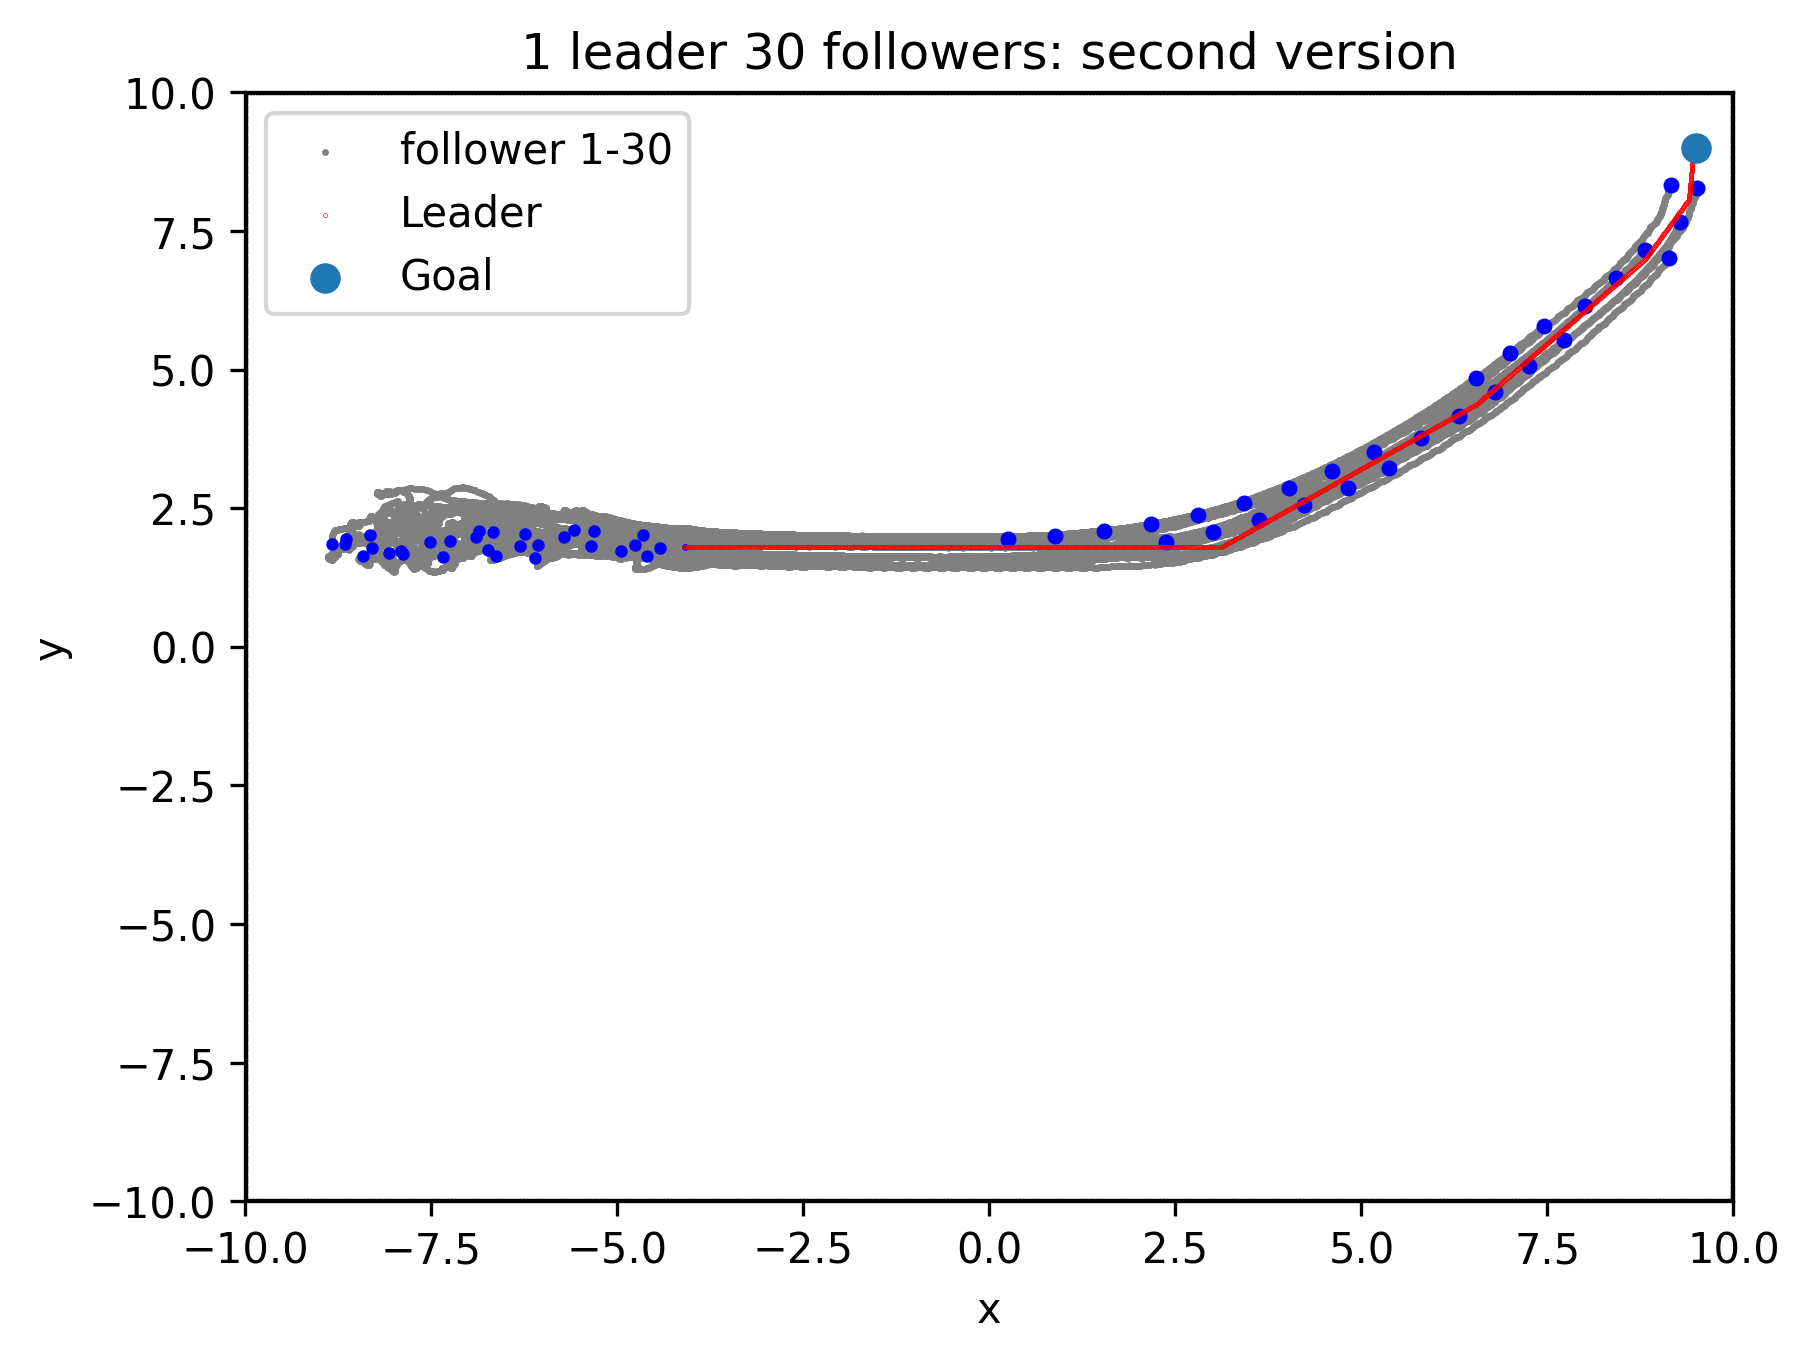
\includegraphics[scale=0.8]{figures/images/results/swarm_second_version.png}
    \caption{30 követő ágens, egy vezér}
    \label{fig:result_30_foll_1_lead}
\end{figure}





%következtetés
\chapter{Összefoglalás}
\section{Összefoglalás}

\addcontentsline{toc}{chapter}{Irodalomjegyzék}
\bibliographystyle{ieeetr}
\bibliography{References}

%appendix
\appendix
\chapter{Függelék}
\section{Alfejezet}

\subsection{Cím}

\subsubsection{Alcím}




\end{document}